\documentclass[10pt,a4paper]{article}
\usepackage[T1]{fontenc}
\usepackage{amsmath}
\usepackage{amssymb}
\usepackage{braket}
\usepackage{graphicx}
\usepackage{float}
\usepackage[a4paper, margin=1.5cm]{geometry}
\usepackage{titlesec}
\usepackage{xcolor}
\usepackage{colortbl}
\usepackage{booktabs}
\usepackage{microtype}
\usepackage{mdframed}
\usepackage{array}

% ── Farben ──────────────────────────────────────────────────────────────
\definecolor{mainblue}{RGB}{10, 60, 120}
\definecolor{accentblue}{RGB}{30, 100, 180}
\definecolor{headerblue}{RGB}{210, 228, 248}
\definecolor{rowalt}{RGB}{240, 245, 252}
\definecolor{ruleline}{RGB}{10, 60, 120}

% ── Abschnittsformatierung ───────────────────────────────────────────────
\titleformat{\section}
{\large\bfseries\color{mainblue}}
{\thesection}{0.8em}{}
[\vspace{-4pt}\textcolor{accentblue}{\rule{\linewidth}{0.8pt}}]

\titleformat{\subsection}
{\normalsize\bfseries\color{accentblue}}
{\thesubsection}{0.8em}{}

\titleformat{\subsubsection}
{\small\bfseries\color{accentblue!80!black}}
{\thesubsubsection}{0.8em}{}

\titleformat{\paragraph}[hang]
{\normalfont\normalsize\bfseries\color{accentblue!70!black}}
{\theparagraph}{1em}{}

% ── Tabellen-Hilfsmakros ─────────────────────────────────────────────────
% Einheitliche Spaltenbreite
\newcolumntype{F}{p{0.3\textwidth}}

% Farbige Kopfzeile in Tabellen
\newcommand{\thead}[1]{\cellcolor{headerblue}\textbf{#1}}

% Trennlinie in Tabellenfarbe
\arrayrulecolor{accentblue}

% ── Dokument ─────────────────────────────────────────────────────────────
\title{\textbf{\color{mainblue}Formelsammlung Physik}}
\date{November 10, 2025}
\author{Noe Schmutz, Sven Pfister, Joel Rechsteiner, Nils Kreienbühl \\
	\small ZHAW School of Engineering – Systemtechnik PHY1}

\begin{document}
	
	%\maketitle
	\tableofcontents
	\bigskip
	\pagebreak
	
	% ════════════════════════════════════════════════════════════════════════
	\section{Kinematik}
	% ════════════════════════════════════════════════════════════════════════
	
	\subsection{Beschleunigte Bewegung}
	\subsection{Beschleunigung}
	
	\begin{tabular}{FFF}
		\toprule
		\thead{Beschleunigungsgleichungen} & & \\[4pt]
		\midrule
		$a = \dfrac{v - v_0}{t}$ &
		$a = \dfrac{2(s - s_0 - v_0 t)}{t^2}$ & \\[8pt]
		\bottomrule
	\end{tabular}
	
	\subsection{Geschwindigkeit}
	
	\begin{tabular}{FFF}
		\toprule
		\thead{Geschwindigkeitsgleichungen} & & \\[4pt]
		\midrule
		$v = v_0 + a t$ &
		$v^2 - v_0^2 = 2 a s$ &
		$v=\sqrt{2as+v_0}$ \\[6pt]
		\bottomrule
	\end{tabular}
	
	\subsection{Strecke}
	
	\begin{tabular}{FFF}
		\toprule
		\thead{Weg-Zeit-Gleichung} & & \\[4pt]
		\midrule
		$s = s_0 + v_0 t + \tfrac12 a t^2$ &
		$t = \sqrt{\dfrac{2h}{g}}$ & \\[8pt]
		\bottomrule
	\end{tabular}
	
	\subsection{Senkrechter Wurf}
	
	\begin{tabular}{FFF}
		\toprule
		\thead{Zeit bis zum höchsten Punkt} &
		\thead{Zeit bis wieder auf Ausgangshöhe} & \\[4pt]
		\midrule
		$t = \dfrac{v_0}{g}$ &
		$t = \dfrac{2 v_0}{g}$ & \\[8pt]
		\bottomrule
	\end{tabular}
	
	\subsection{Schiefer Wurf}
	
	\begin{tabular}{FFF}
		\toprule
		\thead{Geschwindigkeit in $x$} &
		\thead{Geschwindigkeit in $y$} &
		\thead{Gesamtgeschwindigkeit} \\[4pt]
		\midrule
		$v_x = v_0 \cos\theta$ &
		$v_y = v_0 \sin\theta$ &
		$v_{\text{ges}} = \sqrt{v_x^2 + v_y^2}$ \\[10pt]
		\rowcolor{rowalt}
		\thead{Zeit bis Maximum} &
		\thead{Nur Maximum (Scheitelpunkt)} &
		\thead{Ort nach der Zeit allg.} \\[4pt]
		$t_h = \dfrac{v_y}{g}$ &
		$h=h_0+\dfrac{v_{0y}^2}{2g}$ &
		$h=h_0+v_{0y}\,t-\tfrac{1}{2}\,g\,t^2$ \\[10pt]
		\rowcolor{rowalt}
		\thead{Zeit gesamt} &
		\thead{Strecke gesamt} &
		\thead{Auftreffwinkel} \\[4pt]
		$t_{ges} = t_h + \sqrt{\dfrac{2 h_0}{g}}$ &
		$x_{ges} = v_x\,t_{ges}$ &
		$\tan\alpha = \dfrac{v_y}{v_x}$ \\[10pt]
		\bottomrule
	\end{tabular}
	
	\paragraph{Lösung über Standardgleichung als quadratische Funktion}\mbox{}\\[4pt]
	
	\begin{tabular}{FFF}
		\toprule
		\thead{Standardgleichung} &
		\thead{Null setzen} &
		\thead{Mitternachtsformel} \\[4pt]
		\midrule
		$y(t)=h_0+v_{0y}\,t-\tfrac{1}{2}g\,t^2$ &
		$0=h_0+v_{0y}\,t-\tfrac{1}{2}g\,t^2$ &
		$t=\dfrac{v_{0y}\pm\sqrt{v_{0y}^2+2gh_0}}{g}$ \\[10pt]
		\bottomrule
	\end{tabular}
	
	\paragraph{Lösung über Bahnkurve ohne Zeit}\mbox{}\\[4pt]
	
	\begin{tabular}{FFF}
		\toprule
		\thead{Gleichförmige Bew. nach $t$} &
		\thead{Gleichförmige Beschleunigung} &
		\thead{Mitternachtsformel} \\[4pt]
		\midrule
		$x=(v_0\cos\alpha)\,t \;\Rightarrow\; t=\dfrac{x}{v_0\cos\alpha}$ &
		$y=\tan\alpha\cdot x-\dfrac{g}{2v_0^2\cos^2\!\alpha}\,x^2$ &
		$t=\dfrac{v_{0y}\pm\sqrt{v_{0y}^2+2gh_0}}{g}$ \\[10pt]
		\rowcolor{rowalt}
		\thead{Flugzeit (ohne Starthöhe)} &
		\thead{Maximale Höhe} &
		\thead{Wurfweite (ohne Starthöhe)} \\[4pt]
		$t_{flug}=\dfrac{2v_0\sin\alpha}{g}$ &
		$h_{max}=h_0+\dfrac{v_0^2\sin^2\!\alpha}{2g}$ &
		$R=\dfrac{v_0^2\sin 2\alpha}{g}$ \\[10pt]
		\bottomrule
	\end{tabular}
	
	\subsection{Relative Bewegung}
	TBD
	
	% ════════════════════════════════════════════════════════════════════════
	\section{Dynamik}
	\subsection{Newtonsche Axiome}
	% ════════════════════════════════════════════════════════════════════════
	
	\subsubsection{Erstes Axiom – Trägheitsgesetz}
	Ein Körper bleibt in Ruhe oder bewegt sich geradlinig mit konstanter Geschwindigkeit fort,
	wenn keine resultierende äußere Kraft auf ihn wirkt.
	
	\subsubsection{Zweites Axiom – Aktionsprinzip}
	Die Beschleunigung eines Körpers ist direkt proportional zur auf ihn wirkenden Gesamtkraft,
	wobei die Proportionalitätskonstante der Kehrwert der Masse ist. Es gilt:
	
	\[
	a = \frac{F}{m}
	\qquad\text{mit}\qquad
	F = \sum_i F_i
	\]
	
	\subsubsection{Drittes Axiom – Wechselwirkungsprinzip}
	Wenn zwei Körper miteinander wechselwirken, so ist die Kraft $F_A^{(B)}$,
	die Körper B auf Körper A ausübt, gleich groß, aber entgegengesetzt gerichtet
	der Kraft $F_B^{(A)}$, die Körper A auf Körper B ausübt. Es gilt:
	
	\[
	F_A^{(B)} = -\,F_B^{(A)}
	\]
	
	\subsection{Inertialsysteme und Kräfte}
	
	\subsubsection{Inertialsystem}
	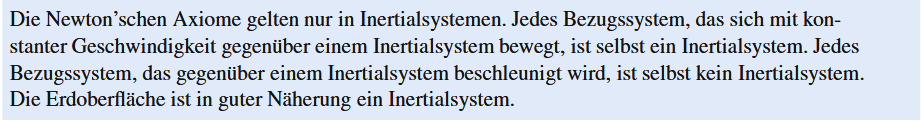
\includegraphics[width=\linewidth]{img/inertialsystem}
	
	\subsubsection{Superposition von Kräften}
	Die Superposition einer Kraft ist die Vektorsumme aller beteiligten Teilkräfte:
	\[
	\vec{F} = \sum_{i=1}^{n} \vec{F}_i
	\]
	
	\subsubsection{Kräftegleichgewicht}
	Beim Kräftegleichgewicht ist die Superposition aller Kräfte gleich null:
	\[
	0 = \vec{F} = \sum_{i=1}^{n} \vec{F}_i
	\]
	
	\subsubsection{Konservative Kräfte}
	Eine Kraft heißt konservativ, wenn die von ihr verrichtete Arbeit beim Bewegen eines Teilchens
	von einem Punkt zum anderen \textbf{unabhängig vom Weg} ist.
	
	\subsection{Normalkraft}
	Das Formelzeichen für die Normalkraft ist $F_{\perp}$ oder $F_N$.
	
	\subsection{Reibungskräfte}
	
	\begin{tabular}{FFF}
		\toprule
		\thead{Haftreibung} &
		\thead{Gleitreibung} &
		\thead{Rollreibung} \\[4pt]
		\midrule
		$F_{R,\text{Haft}} = \mu_H\, F_{\perp}$ &
		$F_{R,\text{Gleit}} = \mu_G\, F_{\perp}$ &
		$F_{R,\text{Roll}} = \mu_R\, F_{\perp}$ \\[6pt]
		\bottomrule
	\end{tabular}
	
	\subsection{Widerstandskräfte}
	
	\begin{tabular}{FFF}
		\toprule
		\thead{Allgemeine Formel} &
		\thead{Beschleunigung} &
		\thead{Endgeschwindigkeit} \\[4pt]
		\midrule
		$F_w = b\, v^{\,n}$ &
		$a_y = -g + \dfrac{b}{m} v^{\,n}$ &
		$v_E = \sqrt[n]{\dfrac{mg}{b}}$ \\[12pt]
		\rowcolor{rowalt}
		\thead{Laminarer Widerstand (Stokes)} & & \\[4pt]
		$F_{\text{Stokes}} = -6\pi\, \mu\, r\, v$ & & \\[6pt]
		\bottomrule
	\end{tabular}
	
	\subsection{Gravitation}
	
	\begin{tabular}{FFF}
		\toprule
		\thead{Gravitationskonstante} &
		\thead{Newtonsche Gravitation} & \\[4pt]
		\midrule
		$\Gamma = 6.6743\cdot 10^{-11}\,\mathrm{N\, m^2\!/kg^2}$ &
		$F_1 = -\,\Gamma\, \dfrac{m_1 m_2}{r^2}$ & \\[10pt]
		\bottomrule
	\end{tabular}
	
	\subsection{Arbeit \& Energie}
	
	\begin{tabular}{FFF}
		\toprule
		\thead{Arbeit} &
		\thead{Kinetische Energie} &
		\thead{Potenzielle Energie} \\[4pt]
		\midrule
		$W=F\cdot s\cdot\cos\alpha$ \newline
		$F=$ Kraft \newline
		$s=$ Strecke \newline
		$\alpha=$ Winkel zw.\ Kraft \& Weg
		&
		$E_{\text{kin}} = \tfrac12 m v^2$
		&
		$E_{\text{pot}} = mgh$
		\\[14pt]
		\rowcolor{rowalt}
		\thead{Mechanische Energie} &
		\thead{Arbeit und Energie} &
		\thead{Gesamtarbeit und kin.\ Energie} \\[4pt]
		$E_{\text{mech}} = E_{\text{kin}} + E_{\text{pot}}$ &
		$W=E_{mech_E}-E_{mech_A}$ &
		$W=\Delta E_{kin}=\tfrac{1}{2}mv_E^2-\tfrac{1}{2}mv_A^2$ \\[10pt]
		\rowcolor{rowalt}
		\thead{Leistung} & & \\[4pt]
		$P = \dfrac{dW}{dt} = F v$ & & \\[6pt]
		\bottomrule
	\end{tabular}
	
	\subsection{Konservative Kräfte}
	
	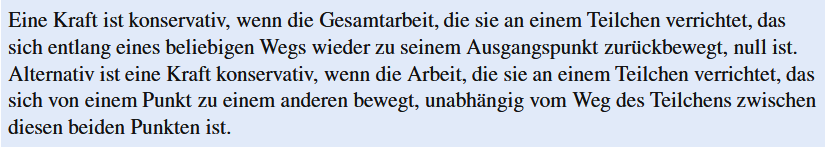
\includegraphics[width=\linewidth]{img/konservative_kräfte}
	
	\subsection{Federn}
	
	\begin{tabular}{FFF}
		\toprule
		\thead{Rückstellkraft} &
		\thead{Arbeit der Feder} &
		\thead{Potentielle Energie} \\[4pt]
		\midrule
		$F_x = -k_F\, x$ &
		$W_{\text{Feder}} = \tfrac12 k_F x_A^2 - \tfrac12 k_F x_E^2$ &
		$E_{\text{Feder}} = \tfrac12 k_F x^2$ \\[6pt]
		\bottomrule
	\end{tabular}
	
	\subsection{Drehbewegung}
	\subsubsection{Rotationsbewegung}
	
	\begin{tabular}{FFF}
		\toprule
		\thead{Frequenz} &
		\thead{Periode} &
		\thead{Winkel} \\[4pt]
		\midrule
		$f = \dfrac{1}{T},\quad [f] = \mathrm{Hz}$ &
		$T = \dfrac{1}{f},\quad [T] = \mathrm{s}$ &
		$\theta \quad [\theta]=\mathrm{rad}$ \\[10pt]
		\rowcolor{rowalt}
		\thead{Strecke} &
		\thead{Winkelgeschwindigkeit (gleichf.)} &
		\thead{Winkelgeschwindigkeit (ungleichf.)} \\[4pt]
		$s = r\theta \quad [s]=\mathrm{m}$ &
		$\omega = \dfrac{\Delta\theta}{\Delta t} = 2\pi f \quad [\omega]=\tfrac{\mathrm{rad}}{\mathrm{s}}$ &
		$\omega = \dfrac{d\theta}{dt} \quad [\omega]=\tfrac{\mathrm{rad}}{\mathrm{s}}$ \\[10pt]
		\rowcolor{rowalt}
		\thead{Winkelbeschleunigung} &
		\thead{Tangentialgeschwindigkeit} &
		\thead{Tangentialbeschleunigung} \\[4pt]
		$\alpha=\dfrac{d\omega}{dt}$ &
		$v_{t,i} = r_i \omega$ &
		$a_t = \dfrac{v_t}{t} = r\dfrac{d\omega}{dt} = r\alpha$ \\[10pt]
		\rowcolor{rowalt}
		\thead{Winkelgeschwindigkeit ohne Zeit} & & \\[4pt]
		$\omega^2 = \omega_0^2+2\alpha(\theta - \theta_0)$ & $\cdot$ & $\cdot$ \\[10pt]
		\rowcolor{rowalt}
		\thead{Zentripetalbeschleunigung} &
		\thead{Zentripetalkraft} & \\[4pt]
		$a_{zp} = |\vec a| = r\omega^2 = \dfrac{v_t^2}{r}$ &
		$F_{zp} = m a_z = m\dfrac{v_t^2}{r} = m\omega^2 r$ & \\[10pt]
		\rowcolor{rowalt}
		\thead{Ortsvektor $\vec r$} &
		\thead{Geschwindigkeit $\vec v$} &
		\thead{Beschleunigung $\vec a$} \\[4pt]
		$\displaystyle\vec r =\begin{pmatrix}r\cos(\omega t)\\r\sin(\omega t)\end{pmatrix}$ &
		$\displaystyle\vec v =\begin{pmatrix}-r\omega\sin(\omega t)\\\;\,r\omega\cos(\omega t)\end{pmatrix}$ &
		$\displaystyle\vec a =\begin{pmatrix}-r\omega^2\cos(\omega t)\\-r\omega^2\sin(\omega t)\end{pmatrix}$ \\[18pt]
		\rowcolor{rowalt}
		\thead{Kraftvektor $\vec F_{\text{ZP}}$} & & \\[4pt]
		$\displaystyle\vec F_{\text{ZP}} = -m\dfrac{v_s^2}{r}\,\hat r = -m r\omega^2\,\hat r$ & & \\[10pt]
		\bottomrule
	\end{tabular}
	
	\subsubsection{Drehmoment}
	
	\begin{tabular}{FFF}
		\toprule
		\thead{Drehmoment} &
		\thead{Arbeit} &
		\thead{Strecke} \\[4pt]
		\midrule
		$\vec M = \vec R \times \vec F$ \\
		$\vec M = \vec I \times \vec \alpha$ (Drallsatz)\\
		$M = F \cdot r \cdot \sin\theta = F \cdot l$ &
		$\vec W = \vec F_{\perp} \times \vec s$ &
		$x = r\,\varphi$ \\[10pt]
		\bottomrule
	\end{tabular}
	
	\subsubsection{Trägheitsmoment}
	
	\begin{tabular}{FFF}
		\toprule
		\thead{Definition Trägheitsmoment} &
		\thead{Kin. Energie rotierender Körper} &
		\thead{Satz von Steiner} \\[4pt]
		\midrule
		$\vec I = \displaystyle\sum_{i} m_i\, r_i^2$ &
		$\vec E_{kin} = \dfrac{1}{2}I\omega^2$ &
		$I = I_S + mh^2$ \\[10pt]
		\bottomrule
	\end{tabular}
	
	\paragraph{Satz von Steiner}
	\noindent
	Wenn ein Körper der Masse m das Trägheitsmoment $I_S$
	bezüglich einer Achse durch den Massenmittelpunkt hat,
	dann ist das Trägheitsmoment I bezüglich einer parallelen Achse im Abstand h von der ersten Achse gegeben
	durch den Steiner’schen Satz.
	
	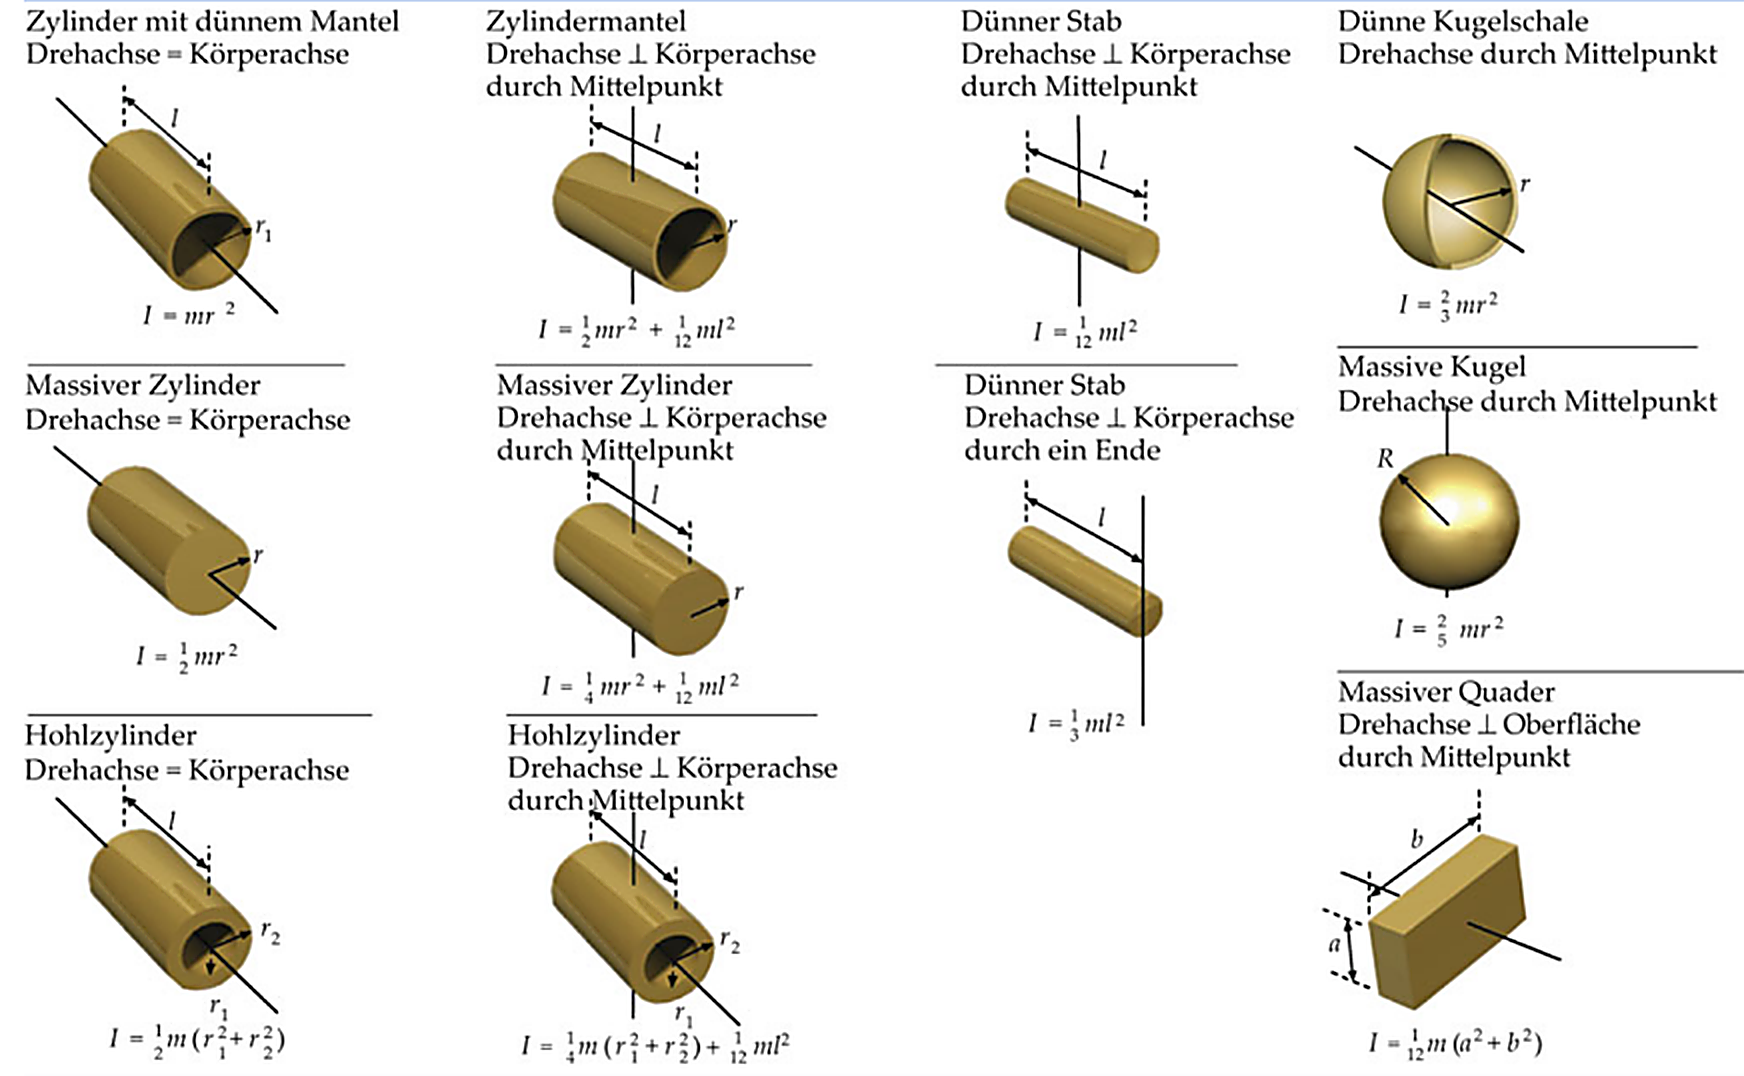
\includegraphics[width=\linewidth]{img/tabelle_trägheitsmoment}
	
	\subsubsection{Drehimpuls}
	
	\begin{tabular}{FFF}
		\toprule
		\thead{Drehimpuls Trägheitsmoment} &
		\thead{Drehimpuls Skalar (x-y-Ebene)} &
		\thead{Drehimpuls bzgl. Symmetrieachse} \\[4pt]
		\midrule
		$L = r \times p = m \vec{r} \times \vec{p}$ &
		$L = m |r||p| \cdot \sin\varphi\;\hat{z}$ &
		$L = I \cdot \omega$ \\[10pt]
		\rowcolor{rowalt}
		\thead{Bahndrehimpuls und Eigendrehimpuls} &
		\thead{Definition des Bahndrehimpulses} & \\[4pt]
		$L = L_{Bahn} + L_{Spin}$ &
		$L_{Bahn} = m r_s \times v_s$ & \\[10pt]
		\bottomrule
	\end{tabular}
	
	\subsubsection{Rollen – Translation \& Rotation}
	
	\begin{tabular}{FFF}
		\toprule
		\thead{Rollbedingung Geschwindigkeit} &
		\thead{Rollbedingung Beschleunigung} &
		\thead{Rollbedingung Distanz} \\[4pt]
		\midrule
		$v = r_P \omega$ &
		$a_s = r \alpha$ &
		$s = r \theta$ \\[10pt]
		\rowcolor{rowalt}
		\thead{Rollbedingung $v$ Massenmittelpunkt} &
		\thead{Kin. Energie rollender Körper} &
		\thead{Geschwindigkeit aus kin. Energie} \\[4pt]
		$v_s = r \omega$ &
		$E_{kin} = \tfrac{1}{2}mv_s^2 + \tfrac{1}{2}I_s\omega^2$ &
		$v=\sqrt{\dfrac{2gh}{1+I_s/(mr^2)}}$ \\[10pt]
		\rowcolor{rowalt}
		\thead{Drehmoment Reibungskraft} &
		\thead{Beschleunigung Starrkörper} &
		\thead{Haftreibung Starrkörper} \\[4pt]
		$M_R = F_R \cdot r = I \cdot \alpha$ &
		$a = \dfrac{m \cdot g \cdot \sin\theta_{\text{Ebene}}}{m + \frac{I}{r^2}}$ &
		$F_R = \dfrac{I\cdot m \cdot g \cdot \sin\theta_{\text{Ebene}}}{I + m \cdot r^2}$ \\[12pt]
		\rowcolor{rowalt}
		\thead{Auflagepunkt unten} &
		\thead{Schwerpunkt Mitte} &
		\thead{Oberster Punkt} \\[4pt]
		$v_{sp} = +v_{sp} - v_{sp} = 0$ &
		$v_{sp} = +v_{sp} + 0 = v_{sp}$ &
		$v_{sp} = +v_{sp} + v_{sp} = 2v_{sp}$ \\[10pt]
		\bottomrule
	\end{tabular}
	
	\pagebreak
	
	% ════════════════════════════════════════════════════════════════════════
	\subsection{Schwingungen}
	% ════════════════════════════════════════════════════════════════════════
	
	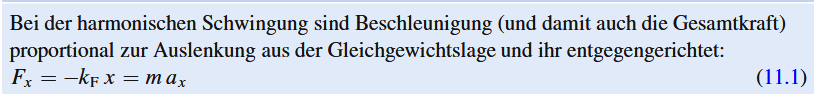
\includegraphics[width=\linewidth]{img/harmonische_schwingung}
	
	\begin{tabular}{FFF}
		\toprule
		\thead{Grundgrößen} &
		\thead{Kreisfrequenz} &
		\thead{Nullphasenwinkel} \\[4pt]
		\midrule
		$\omega =$ Kreisfrequenz \newline
		$A =$ Amplitude \newline
		$\delta =$ Phasenkonstante (Verschiebung) \newline
		$\varphi =$ Phasenwinkel \newline
		$f =$ Frequenz \newline
		$k =$ Federkonstante &
		$\omega = 2\pi f = \sqrt{\tfrac{k}{m}}=\dfrac{2\pi}{T}$ &
		$\varphi_0=\arccos\!\left(\dfrac{x(0)}{A}\right)$ \\[16pt]
		\rowcolor{rowalt}
		\thead{Ort-Zeit-Funktion} &
		\thead{Geschwindigkeit} &
		\thead{Beschleunigung} \\[4pt]
		$x(t)=A\cos(\omega t+\delta)$ \newline
		oder \newline
		$x(t)=A\sin(\omega t+\delta)$ &
		$v(t)=-\omega A\sin(\omega t+\delta)$ \newline
		oder \newline
		$v(t)=\omega A\cos(\omega t+\delta)$ &
		$a(t) = -\omega^2 x(t)$ \\[14pt]
		\rowcolor{rowalt}
		\thead{Potenzielle Energie} &
		\thead{Kinetische Energie} &
		\thead{Gesamtenergie} \\[4pt]
		$E_{pot}(t)=\tfrac12 k_F A^2\cos^2(\omega t+\delta)$ &
		$E_{kin}(t)=\tfrac12 k_F A^2\sin^2(\omega t+\delta)$ &
		$E_{mech}=\tfrac12 k_F A^2$\newline
		$= E_{pot} + E_{kin}$ \\[14pt]
		\rowcolor{rowalt}
		\thead{Mathematisches Pendel – Periode} &
		\thead{Mathematisches Pendel – Frequenz} &
		\thead{Pendel – Kreisfrequenz} \\[4pt]
		$T = 2\pi\sqrt{\tfrac{l}{g}}$ &
		$f = \tfrac{1}{2\pi}\sqrt{\tfrac{g}{l}}$ &
		$\omega = \sqrt{\tfrac{g}{l}}$ \\[10pt]
		\bottomrule
	\end{tabular}
	
	\subsection{Vorgehensweise: Anwendung des zweiten Newtonschen Axioms}
	
	\begin{enumerate}
		\item Zeichnen Sie eine Übersichtsskizze, die alle wichtigen Angaben der Aufgabe zeigt.
		\textbf{Alle Winkel und Winkelgrößen einzeichnen!}
		
		\item Isolieren Sie den zu betrachtenden Körper (das Teilchen) und kennzeichnen Sie alle auf ihn wirkenden Kräfte.
		
		\item Stellen Sie diese Kräfte in einem vollständigen Kräftediagramm dar.
		
		\item Wählen Sie ein zweckmäßiges Koordinatensystem.
		Ist die Richtung des Beschleunigungsvektors bekannt, sollte eine der Koordinatenachsen in diese Richtung gelegt werden.
		
		\item Zerlegen Sie alle Kräfte in ihre Komponenten und zeichnen Sie diese in das Koordinatensystem ein.
		
		\item Wenden Sie das zweite Newtonsche Axiom
		\[
		\sum F_i = m \cdot a
		\]
		für jede Dimension an. Bei Gleichgewicht gilt:
		\[
		\sum F_i = 0,
		\]
		sonst:
		\[
		\sum F_i = m \cdot a.
		\]
		
		\item Lösen Sie die sich ergebenden Gleichungen nach den gesuchten Größen auf.
		
		\item Überprüfen Sie, ob die Ergebnisse die richtigen Maßeinheiten besitzen.
		
		\item Eine gute Möglichkeit zur Fehlerkontrolle ist es, probeweise Grenzwerte
		in die allgemeine Lösung einzusetzen.
	\end{enumerate}
	
	\subsection{Looping}
	
	\begin{table}[H]
		\centering
		\arrayrulecolor{accentblue}
		\begin{tabular}{|l|c|l|}
			\hline
			\rowcolor{headerblue}
			\textbf{Bedeutung} & \textbf{Formel} & \textbf{Bemerkung} \\ \hline
			
			Allgemeine Radialkraftgleichung &
			$\displaystyle N + mg\cos\varphi = \dfrac{mv^2}{r}$ &
			Für beliebigen Winkel $\varphi$ \\ \hline
			
			Normalkraft allgemein &
			$\displaystyle N = \dfrac{mv^2}{r} - mg\cos\varphi$ &
			Umgestellt nach $N$ \\ \hline
			
			Bedingung oben im Looping &
			$\displaystyle mg = \dfrac{mv^2}{r}$ &
			Grenzfall $N=0$ \\ \hline
			
			Minimalgeschwindigkeit oben &
			$\displaystyle v_{\text{oben,min}} = \sqrt{gr}$ &
			Gerade noch Kontakt \\ \hline
			
			Eintrittsgeschwindigkeit unten &
			$\displaystyle v_{\text{unten,min}} = \sqrt{5gr}$ &
			Aus Energieerhaltung \\ \hline
			
			Energieerhaltung allgemein &
			$\displaystyle \tfrac12 mv_1^2 + mgh_1 = \tfrac12 mv_2^2 + mgh_2$ &
			Für zwei beliebige Punkte \\ \hline
			
			Minimal nötige Starthöhe &
			$\displaystyle h_{\min} = \tfrac{5}{2}\, r$ &
			Start aus Ruhe, reibungsfrei \\ \hline
			
			Normalkraft unten &
			$\displaystyle N_{\text{unten}} = mg + \dfrac{mv^2}{r}$ &
			Maximale Belastung \\ \hline
			
			Normalkraft oben &
			$\displaystyle N_{\text{oben}} = \dfrac{mv^2}{r} - mg$ &
			Kann zu $0$ werden \\ \hline
		\end{tabular}
	\end{table}
	
	\subsection{Impuls}
	
	\subsubsection*{Grundlagen}
	\[
	\vec p = m\vec v,
	\qquad
	\vec p_{\rm ges} = \sum_i m_i \vec v_i,
	\qquad
	\vec F = \frac{d\vec p}{dt} \;\Rightarrow\; \vec F = m\vec a \text{ (falls } m=\text{konst.)}
	\]
	
	\subsubsection*{Impulserhaltung}
	\[
	\vec F_{\rm ext}=0 \;\Rightarrow\; \vec p_{\rm ges}=\text{konstant},
	\qquad
	F_{\rm ext,x}=0 \;\Rightarrow\; p_x=\text{konstant}
	\]
	
	\subsubsection*{Kraftstoß}
	\[
	\Delta \vec p = \int_{t_A}^{t_E}\vec F(t)\,dt,
	\qquad
	\langle \vec F\rangle = \frac{\Delta \vec p}{\Delta t}
	\]
	
	\subsubsection*{Kinetische Energie über Impuls}
	\[
	E_{\rm kin}=\frac{p^2}{2m}
	\]
	
	\subsubsection*{Inelastischer Stoß}
	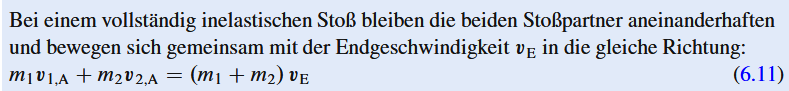
\includegraphics[width=\linewidth]{img/inelastischer_stoss}
	\[
	v_E=\frac{m_1 v_{1,A}+m_2 v_{2,A}}{m_1+m_2}
	\]
	(Impuls erhalten, Energie nicht)
	
	\subsubsection*{Elastischer Stoß (1D)}
	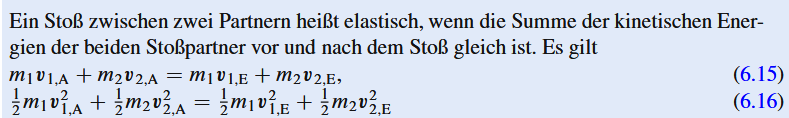
\includegraphics[width=\linewidth]{img/elastischer_stoss}
	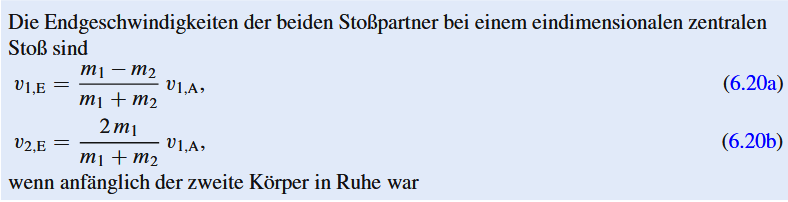
\includegraphics[width=\linewidth]{img/endgeschwindikgeit_elastisch}
	
	\subsubsection*{Relativgeschwindigkeit Elastischer Stoß}
	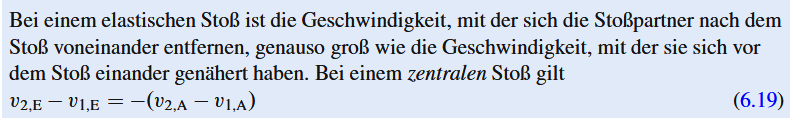
\includegraphics[width=\linewidth]{img/relativgeschwindigkeit_elastischer_stoss}
	
	\subsubsection*{Elastizitätszahl}
	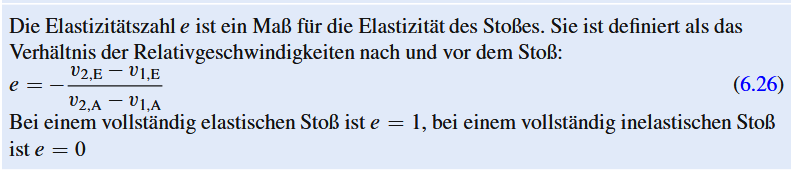
\includegraphics[width=\linewidth]{img/elastizitätzahl}
	
	\subsubsection*{2D-Stöße}
	\[
	\sum p_x=\text{konstant},
	\qquad
	\sum p_y=\text{konstant}
	\]
	(elastisch zusätzlich Energieerhaltung)
	
	\subsubsection*{Massenmittelpunkt}
	\[
	m \cdot r_s = \sum m_i \cdot r_i
	\]
	
	% ════════════════════════════════════════════════════════════════════════
	\subsection{Fluide}
	% ════════════════════════════════════════════════════════════════════════
	
	\begin{tabular}{FFF}
		\toprule
		\thead{Mittlere Dichte} &
		\thead{Definition Dichte} &
		\thead{Dichte von Wasser} \\[4pt]
		\midrule
		$\rho = \dfrac{m}{V} \quad [\rho]\;\dfrac{\mathrm{kg}}{\mathrm{m}^3}$ &
		$\rho = \dfrac{dm}{dV}$ &
		$\rho_{\text{Wasser}} = 1\,\dfrac{\mathrm{g}}{\mathrm{cm}^3} = 1000\,\dfrac{\mathrm{kg}}{\mathrm{m}^3}$ \\[12pt]
		\rowcolor{rowalt}
		\thead{Druck} &
		\thead{Druck (Linearität)} &
		\thead{Auftriebskraft} \\[4pt]
		$P = \dfrac{F}{A} \quad [P]\;\dfrac{\mathrm{N}}{\mathrm{m}^2}$ &
		$p = p_0 + \rho \cdot g \cdot \Delta h$ &
		$F_A=m\cdot g = \rho \cdot V \cdot g$ \\[12pt]
		\rowcolor{rowalt}
		\thead{Maßeinheiten Druck} &
		\thead{Kontinuitätsgleichung – Volumenstrom} &
		\thead{Volumenstrom} \\[4pt]
		$1\,\mathrm{Pa} = 1\,\mathrm{N/m^2} = 10^{-5}\,\mathrm{Bar}$\newline
		$1\,\mathrm{atm} = 101325\,\mathrm{Pa}$ &
		$I_v = A_1 \cdot v_1 = A_2 \cdot v_2 = \mathrm{const}$ &
		$I_v = A \cdot v = \dfrac{V}{t}$ \\[14pt]
		\rowcolor{rowalt}
		\thead{Bernoulli-Gleichung} &
		\thead{Torricelli'sche Ausflussformel} &
		\thead{Venturi-Effekt} \\[4pt]
		$p_1 + \rho g h_1 + \tfrac{1}{2}\rho v_1^2$\newline
		$= p_2 + \rho g h_2 + \tfrac{1}{2}\rho v_2^2 = \mathrm{const}$\newline
		$p$: \textbf{statischer Druck}\newline
		$\rho g h$: \textbf{hydrostatischer Druck}\newline
		$\tfrac{1}{2}\rho v^2$: \textbf{dynamischer Druck} &
		$v=\sqrt{2g\,\Delta h}$ &
		$p + \tfrac{1}{2}\rho v^2 = \mathrm{const}$ \\[14pt]
		\bottomrule
	\end{tabular}
	
	\medskip
	\subsubsection{Pascalsches Prinzip}
	Die Druckänderung eines in einem Behältnis eingeschlossenen Fluids teilt sich unverändert
	jedem Punkt innerhalb des Fluids und den Wänden des Behältnisses mit.
	
	\medskip
	\subsubsection{Barometrische Höhenformel}
	$p=p_0\cdot e^{-\frac{h}{h_0}}$
	
	\medskip
	\subsubsection{Archimedisches Prinzip}
	Ein Körper, der ganz oder teilweise in ein Fluid eintaucht, erfährt eine Auftriebskraft,
	deren Betrag gleich der Gewichtskraft der durch den Körper verdrängten Fluidmenge ist.
	
	\subsubsection{Venturi Effekt}
	Wenn ein Fluid durch eine Verengung strömt, nimmt die
	Strömungsgeschwindigkeit des Fluids zu und der Druck
	ab.
	
	% ════════════════════════════════════════════════════════════════════════
	\subsection{Magnetfeld}
	% ════════════════════════════════════════════════════════════════════════
	
	\begin{tabular}{@{}ll@{}}
		$B$ & magnetische Flussdichte \\
		$\mu_0$ & magnetische Feldkonstante: $4\pi \cdot 10^{-6}\,\tfrac{\mathrm{VS}}{\mathrm{AM}}$ \\
		$I$ & Strom durch Leiter \\
		$r$ & Abstand vom Leiter \\
		$j$ & Stromdichte \\
	\end{tabular}
	
	\[
	F=\mu_0 \frac{I\cdot i}{2\pi r}\,l = B\,i \cdot I
	\qquad
	B = \mu_0 \frac{I}{2 \pi r}
	\]
	
	\subsubsection*{Ampèresches Gesetz}
	\[
	\oint \vec{B} \cdot d\vec{s} = \mu_0 I_{\text{encl}}
	\qquad
	\oint \vec{B} \cdot d\vec{s} = \vec{B} \cdot \oint d\vec{s} = B \cdot 2\pi r
	\qquad
	B(r) = \mu_0 \frac{I}{2\pi r}
	\]
	
	\subsubsection*{Strom}
	\[
	I_{\text{encl}} = j \cdot A(r) = I\,\frac{\pi r^2}{\pi R^2}
	\qquad
	B \cdot S = I
	\]
	
	\subsubsection*{Lorentzkraft}
	
	\begin{tabular}{@{}ll@{}}
		$\vec{F}_L$ & Lorentzkraft \\
		$q$         & bewegte Ladung \\
		$\vec{v}$   & Geschwindigkeit der Ladung \\
		$\vec{B}$   & magnetische Flussdichte \\
		$\alpha$    & Winkel zwischen $\vec{v}$ und $\vec{B}$ \\
	\end{tabular}
	
	\[
	\vec{F}_L = q(\vec{v}\times\vec{B})
	\qquad
	F_L = q \cdot v \cdot B \cdot \sin\alpha
	\qquad
	\vec{F} = I \cdot \vec{l} \times \vec{B}
	\]
	
\end{document}